\title{Decentralised location proof system}

\documentclass[12pt,titlepage]{article}

\usepackage{tikz}
\usetikzlibrary{calc,arrows}
\usepackage{enumitem}
\usepackage{float}

\author{Conor Taylor}
\date{
	B.A.(Mod.) Computer Science\\
	Final Year Project, April 2016\\
	Supervisor: Stephen Barrett
}

\begin{document}
\maketitle

\begin{abstract}
\end{abstract}

\section{Project and Motivation}
Location verification is the process of verifying whether a \textit{node} (computer) is physically present at a location it claims to be. Existing location proof systems attept to use centralised, trusted ``authoritive'' nodes to provide proof of another node's location. These approaches require investment in infrastructure, and are subject to privacy violation and denial of service attacks. This project aims to present a \textit{decentralised} solution to this problem. A decentralised location proof system is a system in which there is no ``authoritive source'' trusted and relied upon to provide and store sensitive location information.

This project describes a decentralised location proof system that is capable of operating on \textit{mobile nodes} (mobile devices). I propose a design in which location proofs are obtained using other untrusted mobile nodes as \textit{alibi's}. Proofs will be created as two mobile nodes communicate over an ad-hoc bluetooth network, transfer encrypted location information, and publish it on a public append-only bulletin board, known as a \textit{blockchain}. The decentralised nature of the system means that there is no single point of failure, no entity controlling the security of every node's location proofs, and no entity capable of violating another node's privacy. This is because in a decentralised system, no node is ``in charge'', and no node has more authority in the system than any other node.
\newpage
\section{Background}
\subsection{Proving your location}
As an increasing amount of personal information is accessible on the internet and therefore on mobile devices, the security that existed by requiring physical interaction between humans to transfer sensitive data is lost.

\subsection{Ad-hoc networks}

\subsection{Blockchain}

\subsection{Centralised location proof systems}
Location proof systems are expected to be accurate and tamper-proof. For this reason, existing solutions have chosen to use a central authority to issue proofs, or to regulate proof issuance \cite{brassil, luo, khan}.

A hardware technique \cite{brassil} operates by supplementing existing WiFi access points with \textit{femtocells}. A femtocell is a small cellular antenna that connects to a mobile carrier via the Internet. Location verification over the internet is made possible by determining which femtocell a mobile node is connected to as it transfers data via Wi-Fi. This solution requires investment in additional hardware to supplement existing WiFi access points, and requires access to mobile providers' user database to identify users locations.

The use of a centralised system, like that described by Brassil et al. \cite{brassil}, creates security, privacy and vulnerability issues. An attacker who succeeds in compromising the security of the central server can violate the privacy of the users of the system, and potentially track their location. The central system architecture is also vulnerable, in the sense that a resource availability attack such as a DDoS attack could render the central architecture unavailable, making location verification unavailable.

Luo et al. propose a system that uses Wi-Fi access points (\textit{AP's}) to allow users to create location proofs \cite{luo}. In their system, each access point has a \textit{group signature} and can sign location proofs for requesting users. Users can request a location proof from any access point, and receive a proof encrypted by the AP with the group signature, as shown in figure \ref{fig:luo_transaction}. This can then be submitted to a Verifier.

\begin{figure}[H]
\begin{center}
\resizebox {0.6\columnwidth} {!} {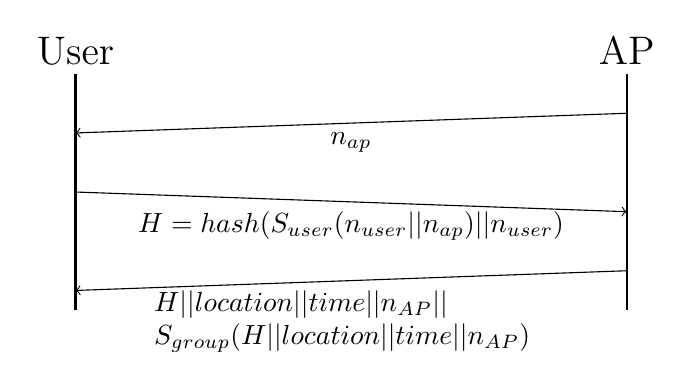
\begin{tikzpicture}
\coordinate (A_T) at (0,3);
\coordinate (A_B) at (0,0);
\coordinate (A_1) at (0,2.25);
\coordinate (A_2) at (0,1.5);
\coordinate (A_3) at (0,0.25);

\coordinate (B_T) at (7,3);
\coordinate (B_B) at (7,0);
\coordinate (B_1) at (7,2.5);
\coordinate (B_2) at (7,1.25);
\coordinate (B_3) at (7,0.5);

\draw[thick] (A_T)--(A_B);
\draw[thick] (B_T)--(B_B);
\draw (A_T) node[above]{\Large User};
\draw (B_T) node[above]{\Large AP};

\draw[->] (B_1) -- (A_1) node[midway,below] {$n_{ap}$};
\draw[->] (A_2) -- (B_2) node[midway,below]
	{$H = hash(S_{user}(n_{user} || n_{ap}) || n_{user})$};
	
\draw[->] (B_3) -- (A_3) node[text width=5cm,midway,below]
	{$H || location || time || n_{AP} ||$\\
	$S_{group}(H || location || time || n_{AP})$};
\end{tikzpicture}}
\end{center}
\caption{Adopted from Luo et al. \cite{luo}}
\label{fig:luo_transaction}
\end{figure}

This kind of system creates \textit{proactive} location proofs. A proactive location proof is one which is created before it is needed. The user creates application-independent location proofs, and can use them at a later time with any application(s) he chooses.

\newpage
\begin{thebibliography}{9}

\bibitem{brassil}
  J. Brassil, P.K. Manadhata,
  ``Verifying the Location of a Mobile Device User'',
  Proc. of MobiSec 2012,
  June 2012.

\bibitem{luo}
  Luo, W., Hengartner, U.,
  ``Proving your Location without giving up your Privacy'',
  Proceedings of the Eleventh Workshop on Mobile Computing Systems \& Applications,
  HotMobile 2010, Annapolis, Maryland, February 22 - 23, pp. 7–12. ACM,
  New York (2010)

\bibitem{khan}
  R. Khan, S. Zawoad, M. M. Haque, and R. Hasan,
  ```Who, When, and Where?' Location Proof Assertion for Mobile Devices'',
  Proceedings of the 28th Annual IFIP WG 11.3 Working Conference on Data and Applications Security and Privacy, ser. DBSec. IFIP,
  July 2014.
 
\bibitem{otit}
  Khan, R., Zawoad, S., Haque, M., Hasan, R.
  ``OTIT: Towards secure provenance modeling for location proofs'',
  Proc. of ASIACCS. ACM (2014)

\bibitem{sybil}
  Douceur, J.R.,
  ``The sybil attack'',
  Druschel, P., Kaashoek, M.F., Rowstron, A. (eds.) IPTPS 2002. LNCS, vol. 2429, pp. 251–260,
  Springer, Heidelberg (2002)

\bibitem{location-spoof}
  N. O. Tippenhauer, K. B. Rasmussen, C. Popper, and S. Capkun,
  ``iPhone and iPod location spoofing: Attacks on public WLAN-based positioning systems'',
  SysSec Technical Report,
  ETH Zurich, April, 2008

\end{thebibliography}

\end{document}